% =====================================================================
%  scheduling-captions.tex
%
%  Stand-alone caption blocks for the eight validation panels of
%  "Trajectory Scheduling". Each figure* block may be \input or copied
%  into the main document. Labels match the \cref targets used in the
%  paper's theorem statements.
% =====================================================================

% ---------------------------------------------------------------------
\begin{figure*}[!htbp]
    \centering
    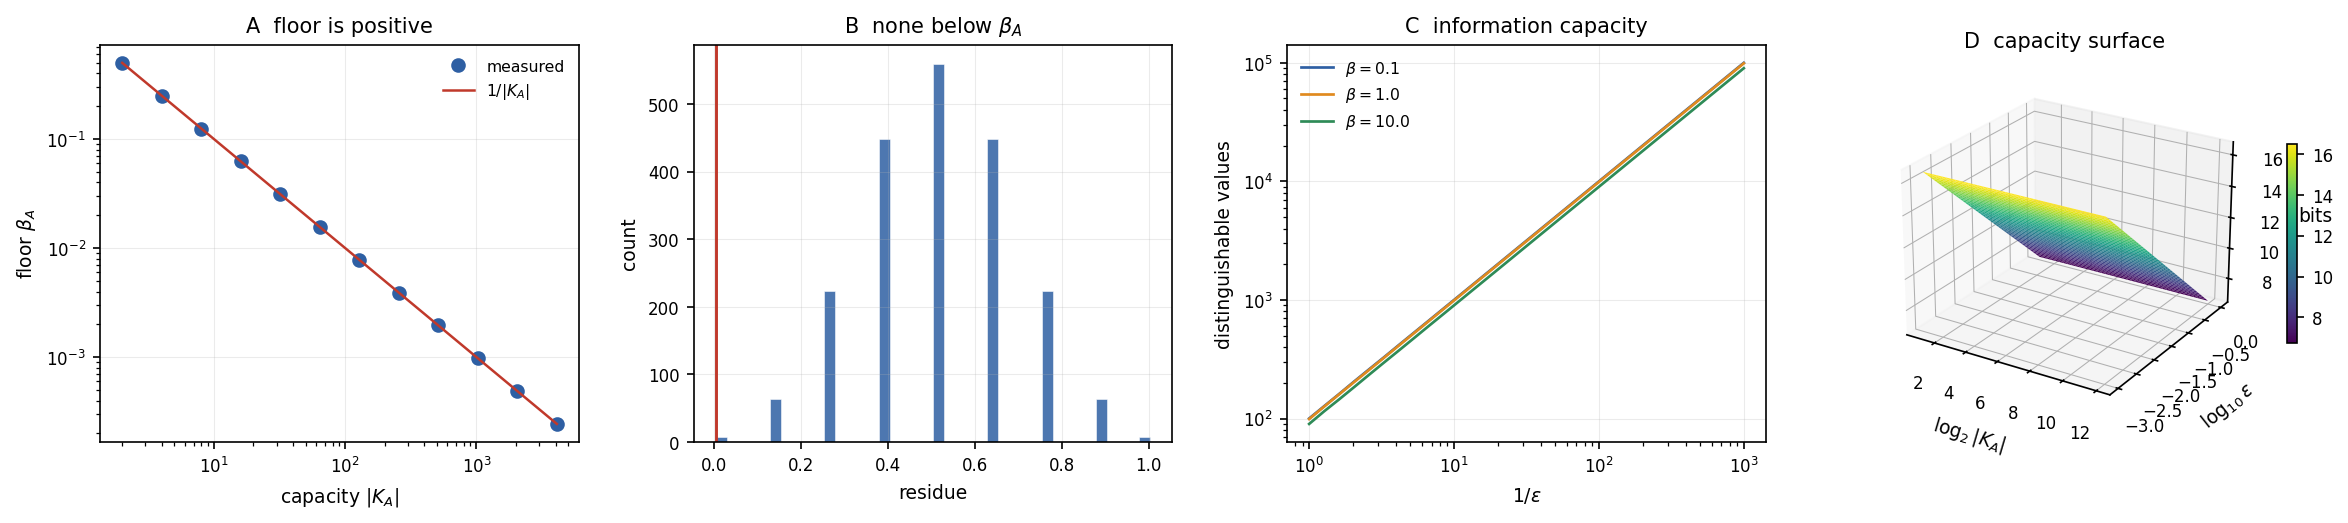
\includegraphics[width=\textwidth]{figures/panel_1.png}
    \caption{\textbf{The Residue Floor and the Information Capacity of the Residue Scale.}
    (\textbf{A})~Measured diagonal floor $\floor_A$ on the logarithmic $y$-axis versus agent capacity $\abs{K_A}$ on the logarithmic $x$-axis for twelve capacities $\abs{K_A}\in\{2,4,8,\dots,4096\}$. Steelblue circles are the floor read from a bounded agent whose encoder collapses $\abs{K_A}\!\cdot\!8$ candidates onto $\abs{K_A}$ internal states; the crimson line is the prediction $\floor_A=1/\abs{K_A}$. The measured floor coincides with $1/\abs{K_A}$ to machine precision at every capacity and is strictly positive throughout, the empirical content of Theorem~\ref{thm:floor} (Residue Floor): a bounded agent cannot resolve a candidate below a strictly positive floor.
    (\textbf{B})~Distribution of the residue read over all $\abs{K_A}\!\cdot\!8$ candidates at capacity $\abs{K_A}=256$ (steelblue bars, white edges), with the floor $\floor_A=1/256$ marked (crimson vertical line). The histogram is supported entirely at and above the floor; no candidate is read below it, confirming the no-candidate-below-floor clause of Theorem~\ref{thm:floor}.
    (\textbf{C})~Number of distinguishable residue values on the logarithmic $y$-axis versus inverse precision $1/\eps$ on the logarithmic $x$-axis, for floors $\floor\in\{0.1,1.0,10.0\}$ (steelblue, orange, green) over $\eps\in[10^{-3},1]$. Each curve is the predicted bound $\lceil(U-\floor)/\eps\rceil$ with $U=100$; the distinguishable-value count rises linearly in $1/\eps$, the content of Theorem~\ref{thm:info} (Information capacity).
    (\textbf{D})~Three-dimensional surface of the residue-scale information content $\log_2\!\big((U-\floor)/\eps\big)$ over $\log_2\abs{K_A}\in[1,12]$ and $\log_{10}\eps\in[-3,0]$, with $\floor=1/\abs{K_A}$ and $U=100$, viridis colourmap, viewing angle elevation $24^{\circ}$ azimuth $-58^{\circ}$. The surface is strictly positive throughout and rises as precision sharpens, displaying the sizing law of Theorem~\ref{thm:info}: distinguishing residue at precision $\eps$ demands the indicated bits of representational capacity.}
    \label{fig:panel1}
\end{figure*}

% ---------------------------------------------------------------------
\begin{figure*}[!htbp]
    \centering
    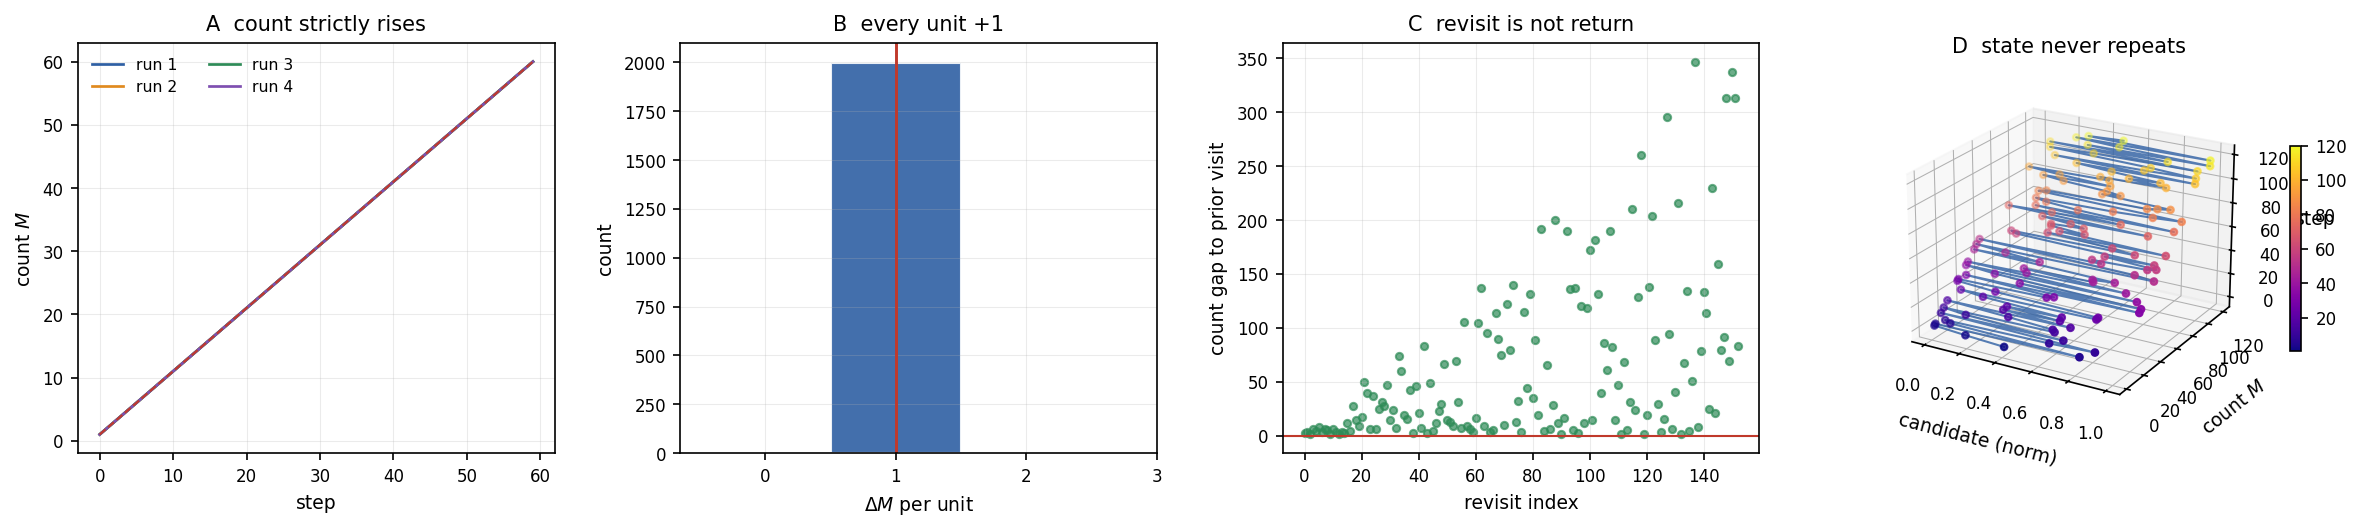
\includegraphics[width=\textwidth]{figures/panel_2.png}
    \caption{\textbf{Strict Monotonicity of the Trajectory Count: an Undo is a Forward Unit.}
    (\textbf{A})~Trajectory count $\Mcount$ on the linear $y$-axis versus committed step on the linear $x$-axis for four independent $60$-step runs (steelblue, orange, green, purple), each with a $30\%$ fraction of ``undo'' units that restore a prior candidate. The crimson dashed line is the ideal $\Mcount=\text{step}$. Every run rises strictly and lies exactly on the diagonal, the empirical content of Theorem~\ref{thm:monotone} (Strict monotonicity): each work unit, undo or not, increments the count.
    (\textbf{B})~Distribution of the per-unit increment $\Delta\Mcount$ over a $2000$-step run including undo operations (steelblue bars, white edges), with the value $1$ marked (crimson vertical line). All mass sits at $\Delta\Mcount=1$: the count never decrements and never jumps, confirming that an undo is itself a counted forward unit.
    (\textbf{C})~Count gap between successive visits of the same candidate on the linear $y$-axis versus revisit index on the linear $x$-axis (green points), over a $400$-step run with $40\%$ undo. Every gap is strictly positive (all points above the crimson line at $0$): a revisited candidate is reached at a strictly larger count, so it is a new state, the content of Corollary~\ref{cor:noreturn} (no return).
    (\textbf{D})~Three-dimensional state path $(\,\text{candidate (normalised)},\,\Mcount,\,\text{step}\,)$ for a $120$-step run with $35\%$ undo, points coloured by count on the plasma scale, viewing angle elevation $22^{\circ}$ azimuth $-60^{\circ}$. The path advances monotonically in the count axis and never returns to a prior $(x,\Mcount)$ state even where the candidate axis repeats, the geometric realisation of Theorem~\ref{thm:monotone} and Corollary~\ref{cor:noreturn}: resemblance of candidate is never identity of state.}
    \label{fig:panel2}
\end{figure*}

% ---------------------------------------------------------------------
\begin{figure*}[!htbp]
    \centering
    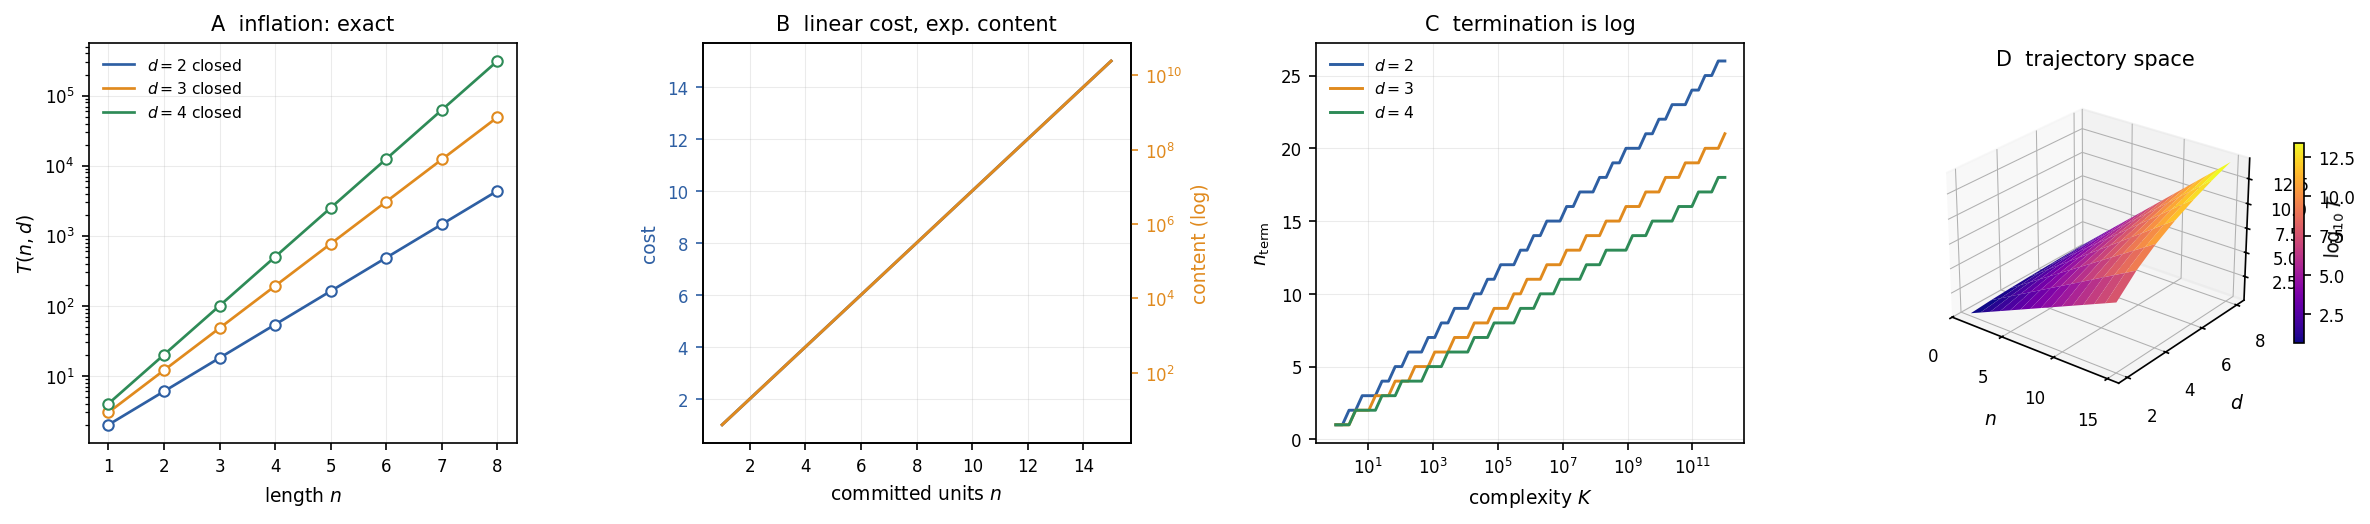
\includegraphics[width=\textwidth]{figures/panel_3.png}
    \caption{\textbf{Trajectory Inflation and the Logarithmic Termination Bound.}
    (\textbf{A})~Distinguishable work-trajectory count $T(n,d)$ on the logarithmic $y$-axis versus length $n\in\{1,\dots,8\}$ on the linear $x$-axis for $d\in\{2,3,4\}$ (steelblue, orange, green). Solid lines are the closed form $T(n,d)=d(d+1)^{n-1}$; open circles are the direct enumeration of compositions of $n$ times $d$-fold type labellings. The two coincide at every $(n,d)$---e.g.\ $T(8,4)=1{,}399{,}680$---the empirical content of Theorem~\ref{thm:inflation} (Trajectory inflation).
    (\textbf{B})~Dual-axis comparison for $d=4$: cumulative cost (steelblue, left linear axis) and distinguishable content $T(n,d)$ (orange, right logarithmic axis) versus committed units $n\in\{1,\dots,15\}$. Cost grows linearly while content grows exponentially, the asymmetry of Remark~\ref{rem:asymmetry}: linear cost, exponential content.
    (\textbf{C})~Termination unit count $n_{\mathrm{term}}(K,d)$ on the linear $y$-axis versus categorical complexity $K$ on the logarithmic $x$-axis for $d\in\{2,3,4\}$ (steelblue, orange, green), $K\in[1,10^{12}]$. Each curve is logarithmic in $K$, e.g.\ $n_{\mathrm{term}}(10^{12},3)=16$; the content of Theorem~\ref{thm:termination} (Logarithmic termination bound).
    (\textbf{D})~Three-dimensional surface of $\log_{10}T(n,d)$ over length $n\in\{1,\dots,15\}$ and type count $d\in\{2,\dots,8\}$, plasma colourmap, viewing angle elevation $26^{\circ}$ azimuth $-52^{\circ}$. The surface rises exponentially in both $n$ and $d$, the trajectory-space inflation that makes content-bounded termination logarithmic (Theorems~\ref{thm:inflation},~\ref{thm:termination}).}
    \label{fig:panel3}
\end{figure*}

% ---------------------------------------------------------------------
\begin{figure*}[!htbp]
    \centering
    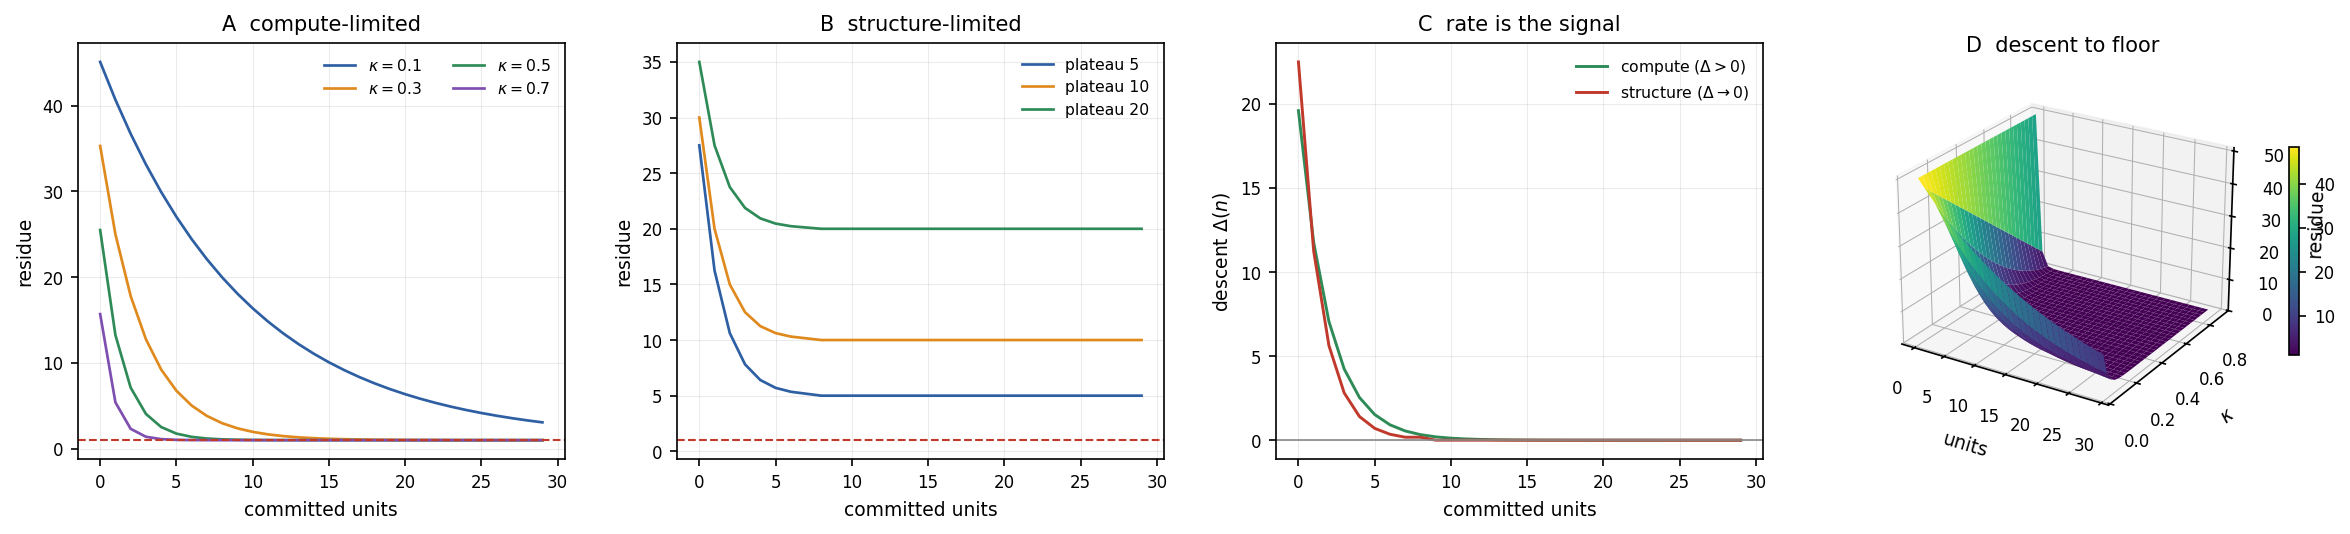
\includegraphics[width=\textwidth]{figures/panel_4.png}
    \caption{\textbf{Runtime Diagnosis: Compute-Limited versus Structure-Limited from the Residue Stream Alone.}
    (\textbf{A})~Residue on the linear $y$-axis versus committed units on the linear $x$-axis for four compute-limited streams with geometric descent rates $\kappa\in\{0.1,0.3,0.5,0.7\}$ (steelblue, orange, green, purple); the floor is marked (crimson dashed). Each stream descends with strictly positive rate $\Delta(n)>0$ toward the floor, the compute-limited regime of Definition~\ref{def:limit} and Theorem~\ref{thm:diagnosis}.
    (\textbf{B})~Residue on the linear $y$-axis versus committed units on the linear $x$-axis for three structure-limited streams that plateau above the floor at levels $\{5,10,20\}$ (steelblue, orange, green); the floor is marked (crimson dashed). After an initial descent the rate $\Delta(n)\to0$ while residue remains strictly above the floor, the structure-limited regime of Definition~\ref{def:limit}.
    (\textbf{C})~Descent rate $\Delta(n)$ on the linear $y$-axis versus committed units on the linear $x$-axis for a representative compute-limited stream (green, $\Delta>0$ sustained) and a structure-limited stream (crimson, $\Delta\to0$), with the zero line marked (grey). The sign of $\Delta(n)$ alone separates the two regimes, the decidability claim of Theorem~\ref{thm:diagnosis}: limit type is read from the residue stream without any running-time estimate.
    (\textbf{D})~Three-dimensional surface of residue $\res = \floor + (50-\floor)(1-\kappa)^{n}$ over committed units $n\in[0,30]$ and descent rate $\kappa\in[0.05,0.9]$, viridis colourmap, viewing angle elevation $24^{\circ}$ azimuth $-58^{\circ}$. The surface descends to the floor for every $\kappa$, the family of compute-limited convergences whose strictly positive $\Delta$ marks them feedable (Theorem~\ref{thm:diagnosis}).}
    \label{fig:panel4}
\end{figure*}

% ---------------------------------------------------------------------
\begin{figure*}[!htbp]
    \centering
    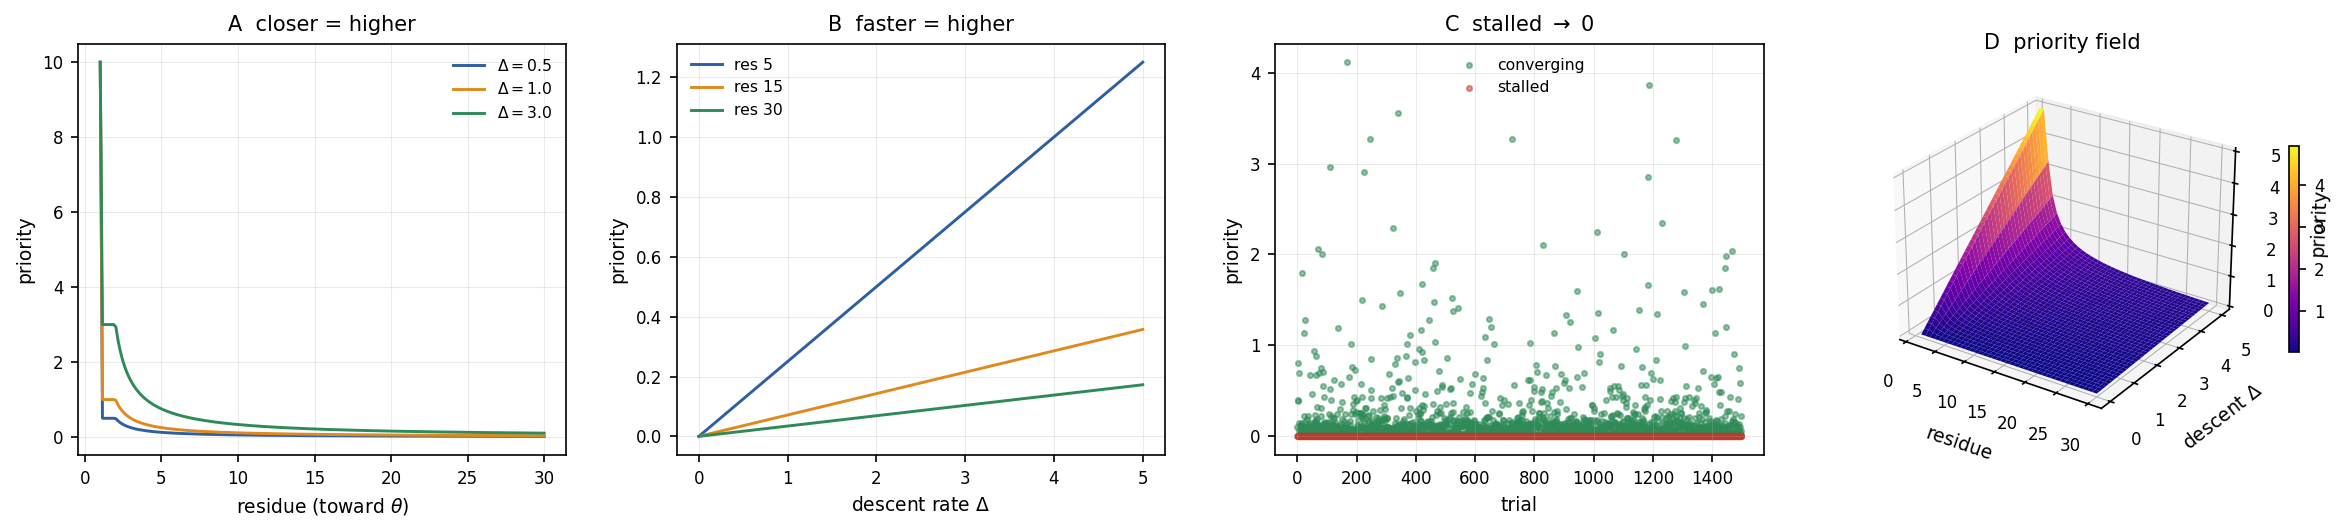
\includegraphics[width=\textwidth]{figures/panel_5.png}
    \caption{\textbf{Residue Priority and Scheduler Soundness.}
    (\textbf{A})~Priority $P(\task)$ on the linear $y$-axis versus residue (approaching the threshold $\theta$) on the linear $x$-axis for descent rates $\Delta\in\{0.5,1.0,3.0\}$ (steelblue, orange, green), clipped at $10$. Priority rises as a task approaches its threshold, the closeness term of Definition~\ref{def:priority}: a nearly-done task is worth finishing.
    (\textbf{B})~Priority $P(\task)$ on the linear $y$-axis versus descent rate $\Delta$ on the linear $x$-axis for residues $\{5,15,30\}$ (steelblue, orange, green). Priority rises linearly in the descent rate, the rate term of Definition~\ref{def:priority}: a fast-converging task is worth advancing.
    (\textbf{C})~Priority on the linear $y$-axis versus trial index on the linear $x$-axis for $1500$ randomly drawn task pairs: converging tasks (green, $\Delta\in[0.01,5]$) and stalled tasks (crimson, $\Delta=0$). Every stalled task has priority $0$ and none out-prioritises a converging task, the empirical content of Theorem~\ref{thm:sound} (Priority-rule soundness): a stalled task is never fed.
    (\textbf{D})~Three-dimensional priority field $P=\Delta/\max(\res-\theta,\floor_A)$ over residue $\res\in[1.01,30]$ and descent rate $\Delta\in[0,5]$ (clipped at $5$), $\theta=1$, plasma colourmap, viewing angle elevation $26^{\circ}$ azimuth $-56^{\circ}$. Priority is zero along the $\Delta=0$ edge (stalled) and grows toward the high-rate, low-residue corner (converging and close), the geometric realisation of Definition~\ref{def:priority} and Theorem~\ref{thm:sound}.}
    \label{fig:panel5}
\end{figure*}

% ---------------------------------------------------------------------
\begin{figure*}[!htbp]
    \centering
    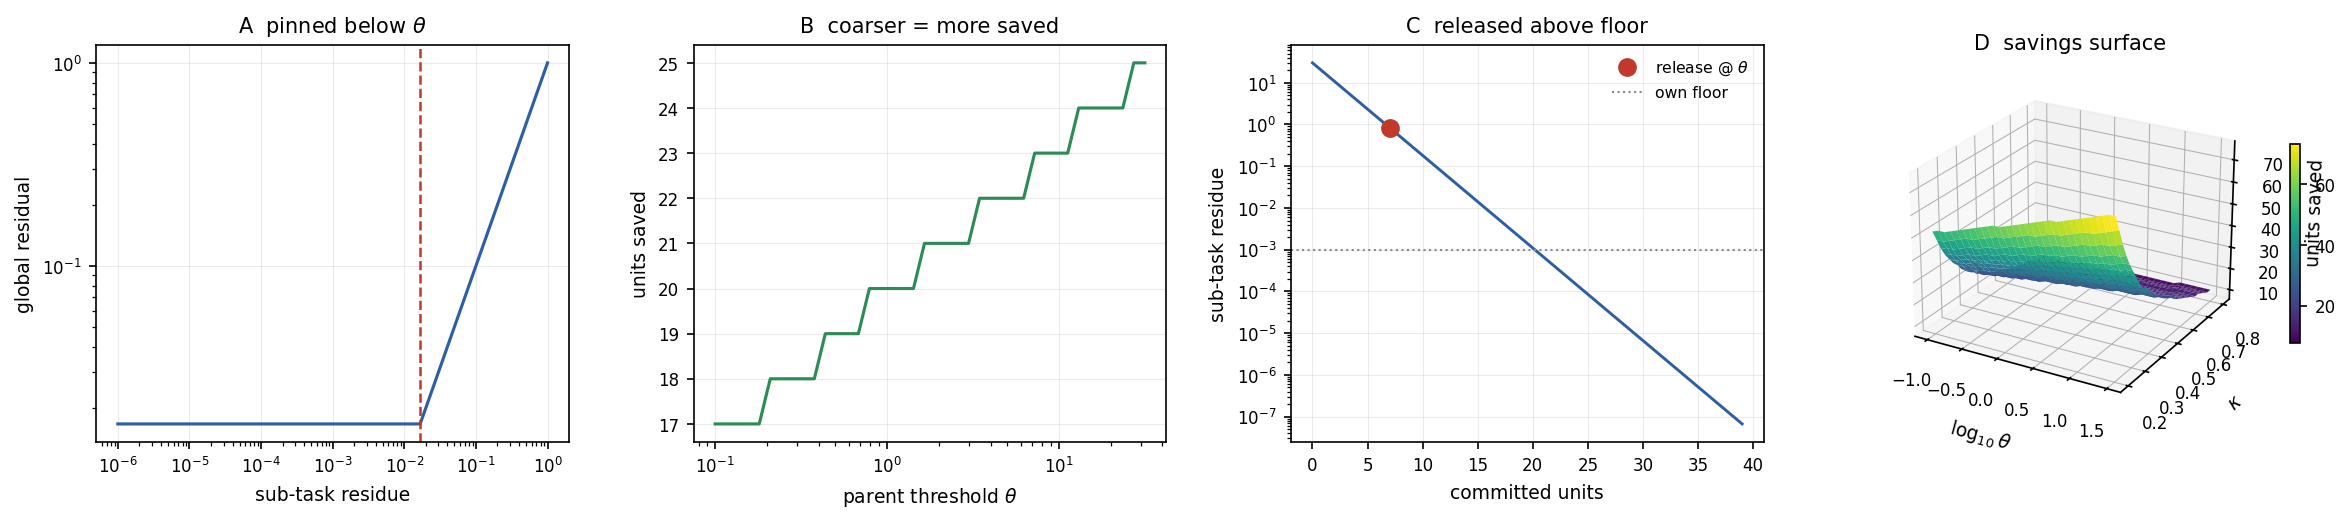
\includegraphics[width=\textwidth]{figures/panel_6.png}
    \caption{\textbf{Sufficiency Stopping: a Sub-Task Released Above its Own Floor.}
    (\textbf{A})~Global residual on the logarithmic $y$-axis versus sub-task residue on the logarithmic $x$-axis, with the parent threshold $\theta=1/60$ marked (crimson dashed), over sub-task residues $[10^{-6},1]$. The global residual equals $\max(\theta,\res_{\text{sub}})$ and is pinned at $\theta$ once the sub-task crosses the threshold, the empirical content of Theorem~\ref{thm:sufficiency}: reducing the sub-task below $\theta$ does not improve the global residual.
    (\textbf{B})~Committed units saved on the linear $y$-axis versus parent threshold $\theta$ on the logarithmic $x$-axis (green), for geometric descent $\kappa=0.5$ from start $50$ to a sub-task floor $10^{-6}$. The saved-unit count grows as the parent threshold coarsens, quantifying the cost spared by releasing at $\theta$ rather than the sub-task's own floor (Theorem~\ref{thm:sufficiency}, Example~\ref{ex:timetable}).
    (\textbf{C})~Sub-task residue on the logarithmic $y$-axis versus committed units on the linear $x$-axis (steelblue), with the release point at $\theta=1$ marked (crimson circle) and the sub-task's own floor at $10^{-3}$ marked (grey dotted). The task is released at $\theta$, strictly above its own attainable floor; the residue it could still reduce is never computed, the content of Theorem~\ref{thm:sufficiency}.
    (\textbf{D})~Three-dimensional surface of committed units saved over $\log_{10}\theta\in[-1,1.5]$ and descent rate $\kappa\in[0.2,0.8]$ (closed-form geometric, start $50$, sub-task floor $10^{-6}$), viridis colourmap, viewing angle elevation $24^{\circ}$ azimuth $-60^{\circ}$. Savings grow as the parent floor coarsens and as descent slows, the surface form of the sufficiency-stopping economy (Theorem~\ref{thm:sufficiency}).}
    \label{fig:panel6}
\end{figure*}

% ---------------------------------------------------------------------
\begin{figure*}[!htbp]
    \centering
    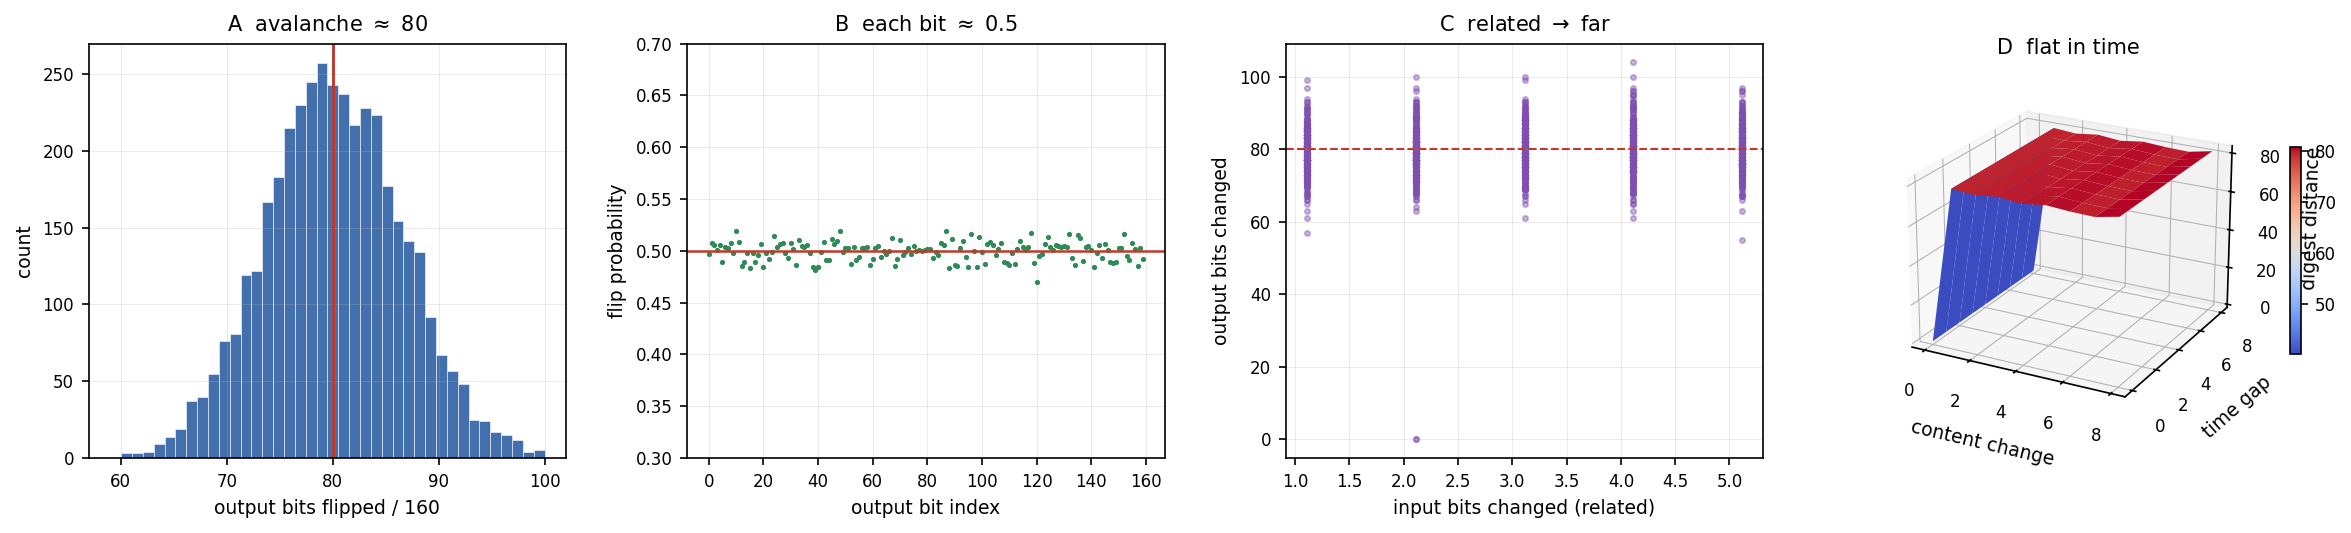
\includegraphics[width=\textwidth]{figures/panel_7.png}
    \caption{\textbf{Avalanche and Time-Blindness of a Content Digest.}
    (\textbf{A})~Distribution of the output Hamming distance (out of $160$ \textsf{SHA-1} bits) induced by a single input-bit flip, over $4000$ random $32$-byte inputs (steelblue bars, white edges), with the half-width value $80$ marked (crimson vertical line). The distribution concentrates at $\approx80$ bits: a minimal (maximally related) input difference produces a near-half output difference, the empirical content of Theorem~\ref{thm:orthogonality} (Label orthogonality) via the strict avalanche criterion.
    (\textbf{B})~Per-output-bit flip probability on the linear $y$-axis versus output bit index $0$ to $159$ on the linear $x$-axis (green points), measured over $3000$ single-bit input flips, with the value $0.5$ marked (crimson line) and the $y$-axis restricted to $[0.3,0.7]$. Every output bit flips with probability $\approx0.5$, the strict avalanche criterion that makes a digest identity-faithful and, by Theorem~\ref{thm:orthogonality}, relatedness-destroying.
    (\textbf{C})~Output bits changed on the linear $y$-axis versus number of input bits changed ($1$ to $5$, jittered) on the linear $x$-axis (purple points, $1500$ trials), with the half-width $80$ marked (crimson dashed). The output difference is $\approx80$ regardless of how few input bits differ: related inputs map to maximally distant digests (Corollary~\ref{cor:no-related}).
    (\textbf{D})~Three-dimensional surface of mean digest distance over content change ($0$ to $8$ input bits flipped) and time gap ($0$ to $8$ trajectory-count units), coolwarm colourmap, viewing angle elevation $22^{\circ}$ azimuth $-62^{\circ}$. The surface rises with content change but is flat along the time-gap axis: the digest is a function of content alone, the empirical content of Theorem~\ref{thm:timeblind} (Time-blindness)---temporal proximity is invisible to a content hash.}
    \label{fig:panel7}
\end{figure*}

% ---------------------------------------------------------------------
\begin{figure*}[!htbp]
    \centering
    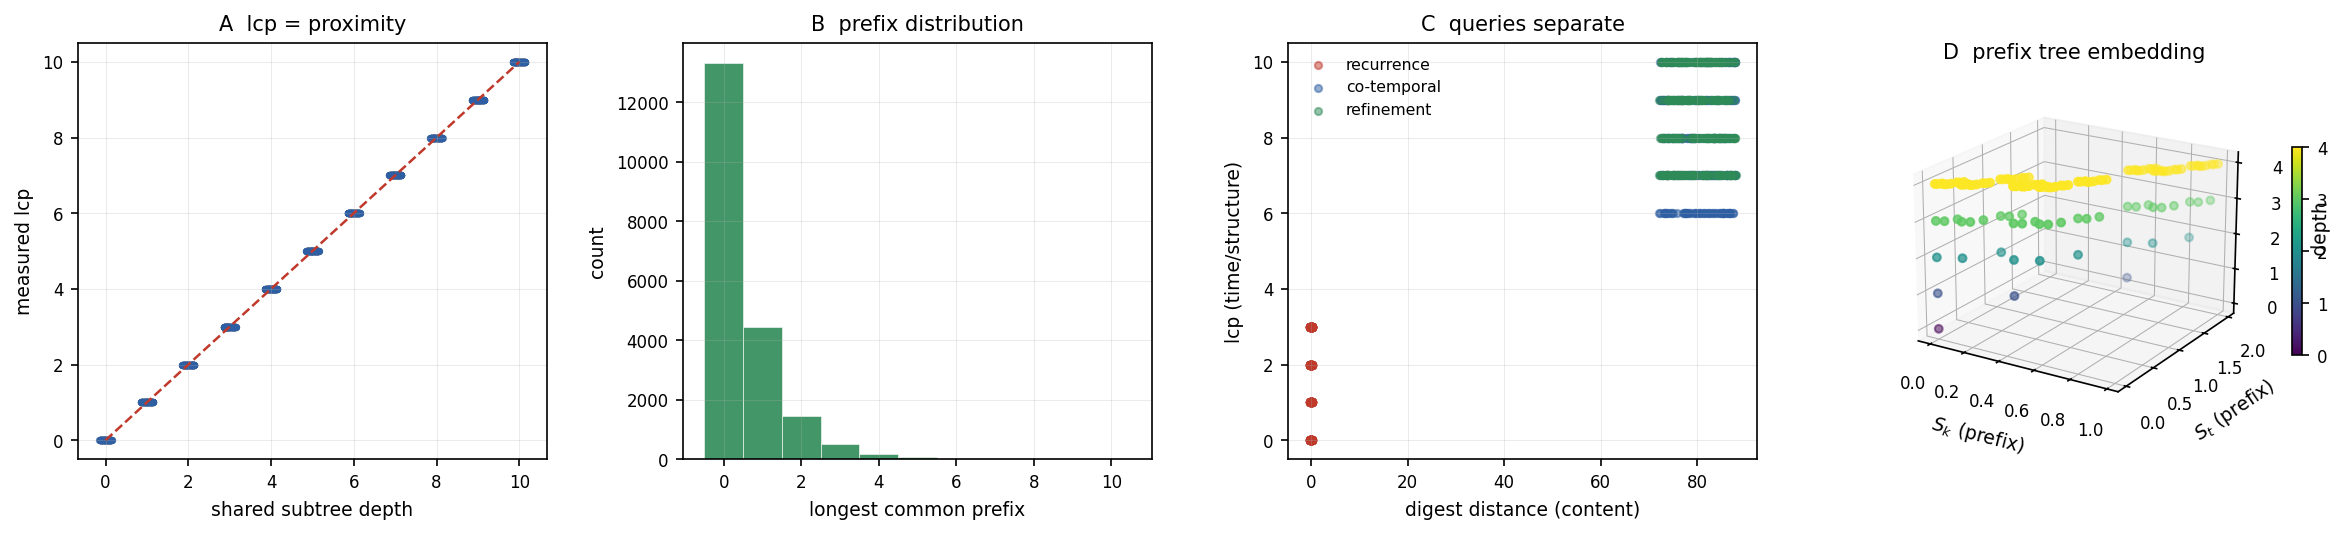
\includegraphics[width=\textwidth]{figures/panel_8.png}
    \caption{\textbf{Prefix is Proximity and the Paired Content--Time Label.}
    (\textbf{A})~Measured longest-common-prefix on the linear $y$-axis versus the constructed shared-subtree depth on the linear $x$-axis (steelblue points, jittered, $4000$ leaf pairs in a depth-$10$ base-$3$ work-tree), with the identity diagonal marked (crimson dashed). Every point lies on the diagonal: the longest common prefix equals the depth of the leaves' lowest common ancestor, the empirical content of Theorem~\ref{thm:prefix}(i) (prefix is proximity).
    (\textbf{B})~Distribution of the longest common prefix over $20{,}000$ random leaf pairs in a base-$3$ depth-$10$ tree (green bars, white edges). The mass concentrates at small prefixes, the geometric base-$b$ profile expected when unrelated leaves share short prefixes; it is the background against which a large prefix certifies genuine structural proximity (Theorem~\ref{thm:prefix}).
    (\textbf{C})~The three relatedness queries in the $(\text{digest distance},\,\text{lcp})$ plane: recurrence (crimson, digest distance $0$, small lcp), co-temporality (steelblue, large digest distance, large lcp), and refinement (green, large digest distance, large lcp), $300$ points each. The queries occupy disjoint regions, the empirical content of Theorem~\ref{thm:queries} (decidable queries): each is decided by a constant number of comparisons on the paired label.
    (\textbf{D})~Three-dimensional embedding of a depth-$4$ base-$3$ address tree: each node placed at $(S_k,S_t)$ from the base-$3$ digit-path expansion of its address, height equal to tree depth, points coloured by depth on the viridis scale, viewing angle elevation $20^{\circ}$ azimuth $-58^{\circ}$. Nodes sharing an address prefix cluster spatially and stack by depth, the geometric realisation of Theorem~\ref{thm:prefix}: shared prefix is shared structural position, the relatedness face of the paired label (Construction~\ref{con:paired}).}
    \label{fig:panel8}
\end{figure*}
